\section{comparison with other formulations}
\label{sec:comparison-other}

In this section we compare our formulation to some existing ones. To simplify the discussions, we
rely on simple examples to demonstrate some of the common issues that arise in graph clustering, and
to point out similarities / differences between our method and some existing ones. We also present
some experimental results on a synthetic and a real-world data sets to verify that our observatoins
extend beyond demonstrating examples.

%\textcolor{magenta}{aaa---this section is still under construction. in the short paper, the section will be replaced by
%a paragraph in the previous section or a pointer.}
%most relevant works are that of Flake et al. \cite{flake:cut-clustering} and
%that of Nagano et al. \cite{nagano2011size}.  We also point out some issues
%that are known to be  problematic for some common clustering techniques, such
%as modularity \cite{newman2006modularity}, Infomap \cite{rosvall2009map}, and
%conductance \cite{add} minimization, but are circumvented in the current
%formulation.


% k-densest sub-graph
The work of \cite{nagano2011size} uses the idea of principle
sequence~\cite{fujishige80,fujishige05,fujishige-pp-revisited} to give a polynomial-time partial
solution to the NP-hard size-constrained submodular function minimization problem. When applied to
graphical networks, the problem reduces to the densest $k$-subgraph problem, and the proposed
solution can be used to identify a portions of the densest $k$-subgraphs.
%Same as the minimum
%average cost clustering, the method in full generality does not have a precise interpretation in
%specific domains. It is different from our framework, as results in \figref{fig:cnr-2000} show that
%our approach can identify strictly more densest subgraphs.
%
%The work in \cite{nagano2011size} considered the size-constrained minimization problem of a
%submodular function.  To make the comparison more concrete (and brief), we focus on the densest
%subgraph problem. The problem is hard in general, however, as shown in \cite{nagano2011size}, 
%it can be partially solved (i.e., for a subset of sizes) using the same formulation
%\eqref{eq:fhat}--\eqref{eq:fb}
In this case the formulation  in \cite{nagano2011size} is similar to 
\eqref{eq:alpha-beta-community} 
with $\beta = 1$ and the constraint $|C| \geq 1$
absent from \eqref{eq:fhat}, i.e., we exclude the empty
set and \cite{nagano2011size} does not.
%. The difference between the
%\eqref{eq:fab}, i.e., it did not exclude the empty set.
It can be shown that this exclusion allows our formulation to fined more solutions to the densest
$k$-subgraph problem. For instance, 
in the graph in Fig.~\ref{fig:eg-chain}, the densest $2$-subgraph is $\Set{1,2}$, which can be
obtained using our algorithm with $\beta = 1$ and $\alpha \in [4,6)$, see
Example~\ref{eg:chain-community}, but cannot be obtained using the formulation in
\cite{nagano2011size} since the empty set achieves a minimum cost of zero over that range of
$\alpha$.
For the same reason the formulation in \cite{nagano2011size} cannot find any communities when
$f$ is chosen to be the in-cut function, i.e., $\beta = 0$, since the empty set is trivially the
optimal solution with zero size and zero in-cut.

%%%%%%%%%%%%%% figure: cnr2000
\begin{figure}[h!]
  \vspace{-1em}
  \centering
  \def\figsep{.2cm}
  \def\dist{1}
  \def\disty{.9}
  \begin{subfigure}[b]{.24\textwidth}
    \subcaptionbox{Our approach with $\beta = 1$ \label{fig:cnr-2000-ab}}{%
      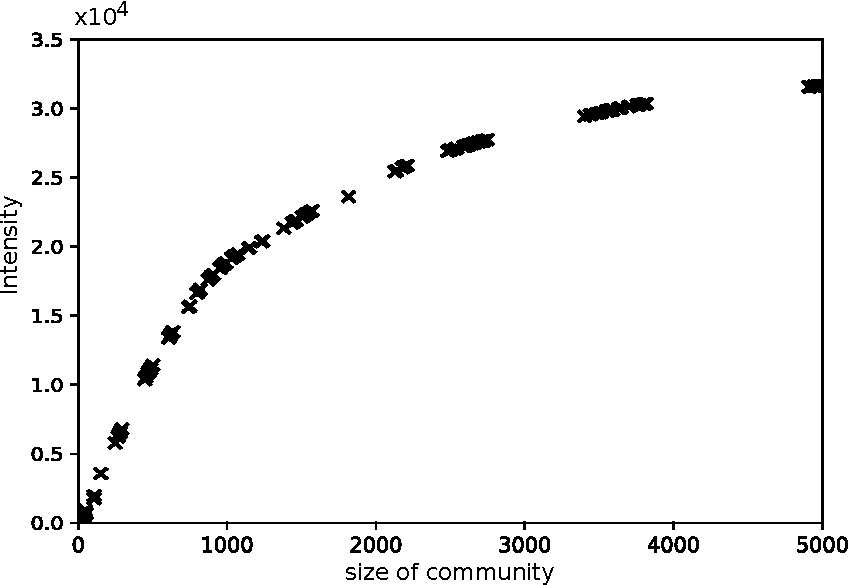
\includegraphics[width=\linewidth]{ab_cnr-2000.pdf}
    }
    % \label{fig:cnr-2000-ab}    
  \end{subfigure}
  \hfill
  \begin{subfigure}[b]{.24\textwidth}
    \subcaptionbox{SSM algorithm. (\cite{nagano2011size})\label{fig:cnr-2000-nagano}}{%
      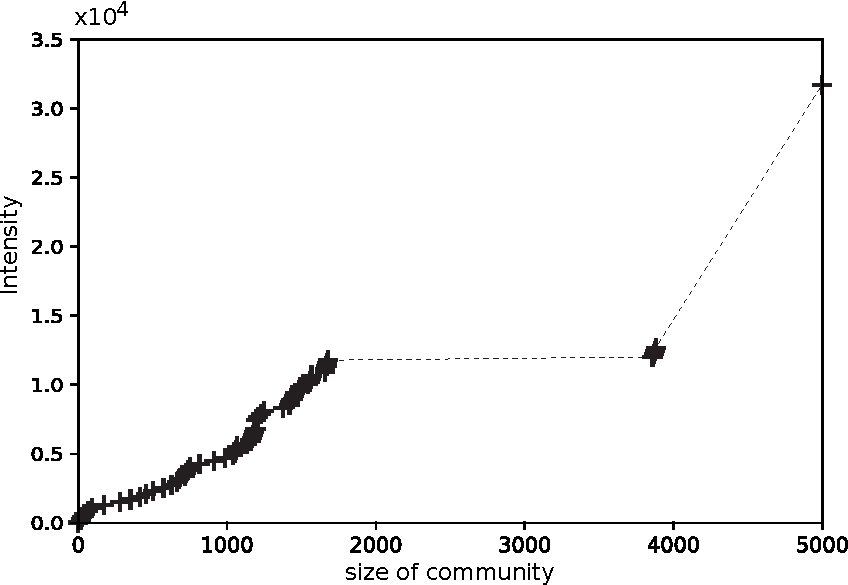
\includegraphics[width=\linewidth]{nagano_cnr-2000.pdf}
    }
    % \label{fig:cnr-2000-nagano}    
  \end{subfigure}
  \caption{Intensity (i.e., total weight of internal edges) versus the size (number of vertices) of
	  the subgraphs returned by (a) our approach and (b) by \cite{nagano2011size}.
	  %Our formulation returns more solutions (densest $k$-subgraphs) than 
	  %plots showing that the proposed algorithm discovers more densest subgraphts of
	  %large sizes. Our method retrieves 51 dense communities with cardinality $>$ 2000 while
	  %the SSM algorithm in \cite{nagano2011size} only finds 2 such communities.}
  }
  \label{fig:cnr-2000}
\end{figure}

%%%%%%%%%%%%%% figure: cnr2000
The observation above extends to larger graphs, which is demonstrated in Fig.~\ref{fig:cnr-2000}.
In this experiment, we applied our algorithm with $\beta = 1$ to the social-network data set
\emph{cnr-2000}, which is a directed unweighted graph. We preprocessed the network in the same way
as \cite{nagano2011size}.
By comparing the result of our algorithm to their proposed SSM algorithm, we are able to retrieve
$51$ dense communities with cardinality larger than $2000$, while \cite{nagano2011size} reported that their SSM algorithm can only find
two such communities.

We remark that a web-community is not necessarily a densest subgraph.\footnote{Not to be confused
	with our discussion in an earlier section where we remarked that a densest subgraph is not necessarily a web-community, e.g., see
	Fig.~\ref{fig:eg-star}.} 
For instance, consider the graph in Fig.~\ref{fig:DSP}.  The set $\{0,1\}$ is a web-community
that is returned by our method, but it is not a densest $2$-subgraph since the subgraph $\{2,3\}$
has strictly more internal support.  Hence, any graph clustering algorithm that only returns densest
subgraphs will fail to return such a web-community.


The modularity \cite{newman2006modularity}, Infomap \cite{rosvall2009map}, and conductance
minimization \cite{shi2000normalized} formulations lead to NP-hard problems, and so rely on
approximations.
Modularity optimization, despite its popularity, has some limitations as pointed out in
\cite{fortunato2007resolution}. One limitation is the resolution limit where the modularity score is tends to favour larger
communities. 
For instance, for the graph in Fig.~\ref{fig:modularity_2} (right), the  modularity score is
minimized by the entire set, and so it fails to detect the more meaningful communities $\Set{0,1}$
and $\Set{2,3}$, which can be identified using our formulation.
Another example is  the ring of cliques \cite{fortunato2007resolution} shown in \ref{fig:modularity_2} (left) for 
$30$ cliques each of size $5$. In this case, the modularity method
groups two consecutive cliques as one cluster, while our formulation can identify every clique.

Methods that are based on conductance minimization may also suffer since they tend to favour solutions of
relatively equal size.\footnote{While this is desirable in some applications, it can also lead to some
undesirable solutions.} An example graph demonstrating this is shown in Fig.~\ref{fig:conductance}.
A similiar issue is faced by Infomap as shown in Figs.~\ref{fig:infomap} and \ref{fig:infomap2}.


Fig. \ref{fig:LFR} shows that many existing methods fail to find strong communities of large sizes
as returned by our proposed methods. The result uses a synthetic graphical network randomly
generated using an existing method. However, this generation targets partitional clustering methods,
and so we expect even more discrepancies when testing on real-world networks that are hierarchical
in nature. It is also an interesting but challenging problem to generate synethetic networks to test
hierarchical clustering methods.



\tikzstyle{cluster}=[fill opacity=0.2,rounded corners,inner sep=0.1em]

\begin{figure}[t]
  \centering
  \tikzstyle{nodestyle}=[inner sep=0.2em,outer sep=0em]
  \tikzstyle{every to}=[every node/.style={font=\scriptsize}]
  \begin{subfigure}[b]{.45\textwidth}
    \centering
    \begin{tikzpicture}
      \matrix (DSP) [matrix of math nodes,column sep=1.2em, row sep=1em, nodes={nodestyle}]
      {
	|(0)| 0 & |(1)| 1 & |(2)| 2 & |(3)| 3 & |(4)| 4 \\
      };
      \draw (0) to node [above] {1} (1) (2) to node [above] {2} (3) to node [above] {1} (4);
      \node[cluster,fill=blue,fit=(0) (1)] {};
      \node[cluster,draw=red,fit=(2) (3)] {};
    \end{tikzpicture}
    \caption{Densest subgraphs: The set $\{0,1\}$ is a web-community that is not a densest $2$-subgraph since $\{2,3\}$ has strictly more internal support.}
    \label{fig:DSP}    
  \end{subfigure}
  %%%%%%%%%%%%%%%
  \hfill
  %%%%%%%%%%%%%%%
  \begin{subfigure}[b]{0.45\textwidth}
    % for drawing ring of clique
    % https://tex.stackexchange.com/questions/223854/drawing-a-ring-of-cliques-in-tikz-graphs/223902#223902
    \newcommand\single[2]{ % #1=labels, #2= n=number of nodes
      \foreach \x in {1,...,#2}{
        \pgfmathsetmacro{\ang}{360/#2}
        \pgfmathparse{(\x-1)*\ang}
        \node[draw,fill=red,circle,inner sep=1pt] (#1-\x) at (\pgfmathresult:4cm) {};
      }
      \foreach \x [count=\xi from 1] in {1,...,#2}{
        \foreach \y in {\x,...,#2}{
          \path (#1-\xi) edge[-] (#1-\y);
        }
      }
    }
    \centering
    \begin{tikzpicture}
    \begin{scope}[local bounding box=scope1]
    %\node at (0,0){$n=5, m=30$};
    \node at (0,0){$30$ cliques};
    \end{scope}
    \foreach \s[count=\si from 0] in {0,45,90,...,360}{
    \begin{scope}[shift={($(scope1) +(\s:2)$)}, scale=0.1,rotate=\s+90]
    \single{\si}{5};
    \end{scope}
    }
    \foreach \i/\j in {1/2,2/3,3/4,4/5,5/6,6/7,7/8}
    \draw (\i-1)--(\j-3);
    %\draw[dotted,thick, outer sep=10pt] (8-1)--(1-3);
	 \def\dd{.13cm}
    \draw[dotted,thick, outer sep=10pt] ([xshift=-\dd, yshift=\dd]8-1.north)--([xshift=\dd, yshift=-\dd]1-3.south);
    \end{tikzpicture}
	 %
	 \hfill
    \begin{tikzpicture}
      \matrix (DSP) [matrix of math nodes,column sep=1.9em, row sep=2em, nodes={nodestyle}]
      {
		|(0)| 0 \\ |(1)| 1 \\ |(2)| 2 \\ |(3)| 3 \\
      };
		\draw (0) to node [left] {1} (1) (1) to node [left, rotate=0] {$0.6$} (2) to node [left] {1} (3);
      \node[cluster,inner sep=.3em,fill=blue,fit=(0) (1)] {};
      \node[cluster,inner sep=.3em,fill=blue,fit=(2) (3)] {};
      \node[cluster,inner sep=.9em, draw=red,fit=(0) (3)] {};
    \end{tikzpicture}
    \caption{Modularity: Two graphs showing modularity's bias towards solutions of larger size.}
    \label{fig:modularity_2}
  \end{subfigure}
  %%%%%%%%%%%%%%%
  \hfill
  %%%%%%%%%%%%%%%
  \begin{subfigure}[b]{.45\textwidth}
    \centering
    \begin{tikzpicture}
      \matrix (con) [matrix of math nodes,column sep=1.2em, row sep=1em, nodes={nodestyle}]
      {
		|(0)| 0 & |(1)| 1 & |(2)| 2 & |(3)| 3 & |(4)| 4 & |(5)| 5 & |(6)| 6 & |(7)| 7 & |(8)| 8 & |(9)| 9\\
      };
      \draw (0) to node [above] {2} (1) to node [above] {0.6} (2) to node [above] {1} (3) to node [above] {1} (4) to node [above] {1} (5) to node [above] {1} (6) to node [above] {1} (7) to node [above] {1} (8) to node [above] {1} (9);
      \node[cluster,fill=blue,fit=(0) (1)] {};
      \node[cluster,draw=red,fit=(0) (1) (2) (3) (4),inner sep=0.4em] {};
      %\node[cluster,draw=red,fit=(5) (6) (7) (8) (9),inner sep=0.4em] {};
    \end{tikzpicture}
    \caption{Minimum conductance: The sets $\{0,1,2,3,4\}$ and $\{5,6,7,8,9\}$ minimize the conductance to $\frac19$. In contrast,
our approach can return the desired cluster
$\{0,1\}$.}
    \label{fig:conductance}    
  \end{subfigure}
  %%%%%%%%%%%%%%%
  \hfill
  %%%%%%%%%%%%%%%
  \begin{minipage}[b]{0.45\textwidth}
  \begin{subfigure}[b]{\textwidth}
    \centering
    \begin{tikzpicture}
      \matrix (con) [matrix of math nodes,column sep=1.2em, row sep=1em, nodes={nodestyle}]
      {
		|(0)| 0 & |(1)| 1 & |(2)| 2 & |(3)| 3 & |(4)| 4 & |(5)| 5 & |(6)| 6 & |(7)| 7 & |(8)| 8 & |(9)| 9\\
      };
      \draw (0) to node [above] {2} (1) to node [above] {0.6} (2) to node [above] {1} (3) to node [above] {1} (4) to node [above] {1} (5) to node [right] {1} (6) to node [above] {1} (7) to node [above] {1} (8) to node [above] {1} (9);
      \node[cluster,fill=blue,fit=(2) (3) (4) (5) (6) (7) (8) (9)] {};
      \node[cluster,draw=red,fit=(2) (3) (4) (5),inner sep=0.4em] {};
      \node[cluster,draw=red,fit=(6) (7) (8) (9),inner sep=0.4em] {};
      %\node[cluster,draw=red,fit=(5) (6) (7) (8) (9),inner sep=0.4em] {};
    \end{tikzpicture}
    \caption{Infomap: The sets $\{0,1\}$, $\{2,3,4,5\}$ and $\{6,7,8,9\}$ optimize the map equation~\cite{rosvall2008maps}. In contrast,
our approach can return the desired cluster $\{2,3,4,5,6,7,8,9\}$.}
    \label{fig:infomap}    
  \end{subfigure}\\
  \begin{subfigure}[b]{\textwidth}
    \centering
    \begin{tikzpicture}
      \matrix (con) [matrix of math nodes,column sep=1.2em, row sep=1em, nodes={nodestyle}]
      {
	|(0)| 0 & |(1)| 1 & |(2)| 2 & |(3)| 3 & |(4)| 4 & |(5)| 5\\
      };
      \draw (0) to node [above] {1} (1) to node [above] {2} (2) to node [above] {1} (3) to node [above] {0.5} (4) to node [above] {1} (5);
      % \node[cluster,fill=blue,fit=(0) (1)] {};
      \node[cluster,draw=red,fit=(0) (1) (2) (3),inner sep=0.4em] {};
      \node[cluster,draw=red,fit=(4) (5),inner sep=0.4em] {};
      %\node[cluster,draw=red,fit=(5) (6) (7) (8) (9),inner sep=0.4em] {};
    \end{tikzpicture}
    \caption{Infomap: will return \{\{0, 1, 2, 3\},\{4, 5\}\} but not the stronger community
	 $\{1,2\}$. In contrast, our formulation returns all of them parameterized by their strengths.}
    \label{fig:infomap2}
  \end{subfigure}
\end{minipage}
  %%%%%%%%%%%%%%%
  \hfill
  %%%%%%%%%%%%%%%
  \vspace{-.5em}
  \caption{Examples of weighted graphs where our formulation (highlighted in blue) can return more meaningful communities
  than existing methods (circulated in red). (Not all communities are highlighted / listed.)}
  \label{fig:eg_for_graphs}
\end{figure}

\begin{figure}
    \centering
    \def\svgwidth{\columnwidth}
    \fontsize{10}{10}\selectfont
    \input{abcomm.pdf_tex}
    \hfill
    \vspace{-.5em}
    \caption{Strength-size plots showing existing algorithms fail to give strong communities of large sizes. We uses an LFR benchmark network~\cite{lancichinetti2009benchmarks} generated with $\mu=0.1$. Each black circle is a community obtain by our method, and the blue lines link to communities obtained by other methods that are smaller and has lower strength. All points below the red line (shaded in grey) are dominated by the trivial community consisting of all the nodes.}

  \label{fig:LFR}
\end{figure}



